\section{Testaufbau und Ergebnisse}
\label{sec:test}
Nachdem die Implementierung des Tools abgeschlossen war, wurde es mit realen Geräten getestet, um es für den Produktiveinsatz rüsten zu können. Hierfür sei unser Dank dem \emph{Zentralen Informatik Dienst (ZID)} (im speziellen Ing. Gonschorowski und DI (FH) Faber) gewidmet, welche uns entsprechende Geräte zur Verfügung gestellt haben.

\subsection{Testaufbau}
Um unsere Tests durchzuführen wurden uns zwei PoE fähige Switches vom ZID zur Verfügung gestellt. Einer hatte keine Abnehmer angeschlossen und hatte 24 Ports und der zweite hatte 48 Ports angeschlossen, wobei an 15 Ports Abnehmer angeschlossen waren (VoIP Telefone). Abbildung \ref{fig:switches} zeigt eine Übersichtsgrafik über den Aufbau.

// TODO: Füge Abbildung über die Switches ein
\begin{figure}[h]
    \centering
    \leavevmode
    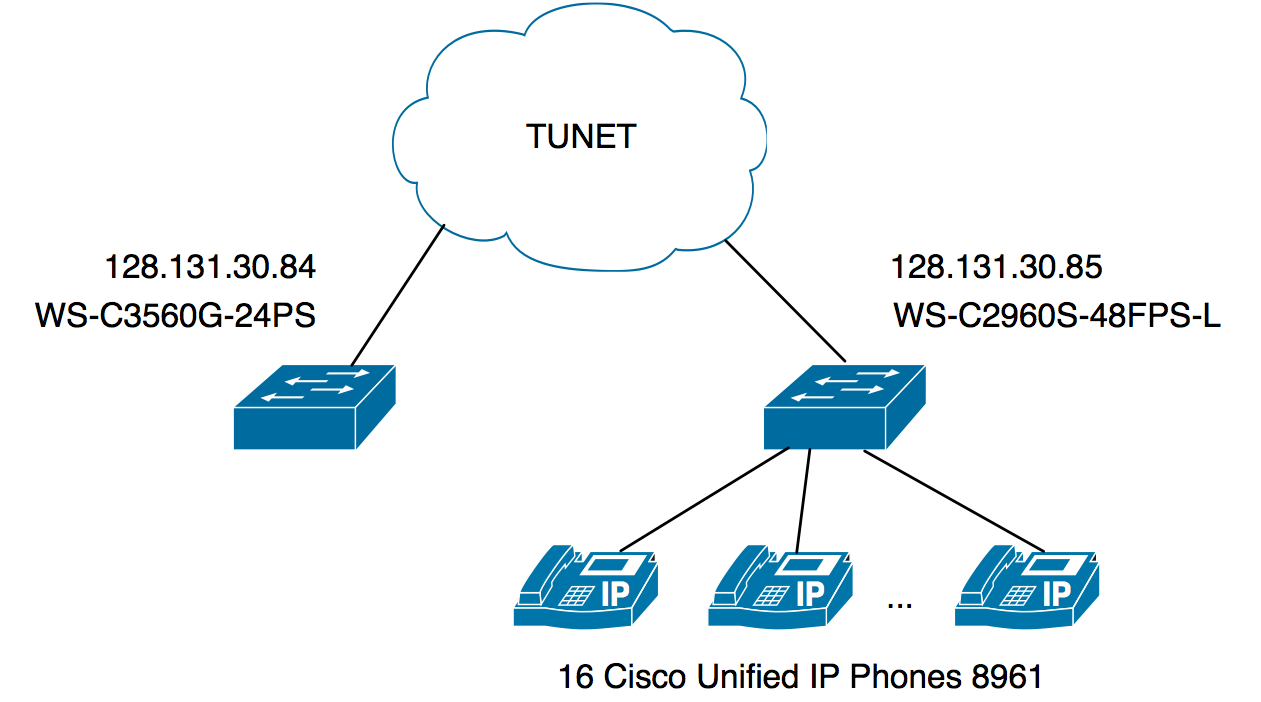
\includegraphics[width=2.0\linewidth]{figures/network_diagram}
    \caption{Abbildung über Switch Aufbau}
    \label{fig:switches}
\end{figure}

Für die Testfälle wurde unser Tool mit den folgenden Einstellungen initialisiert (die Bedeutung der Einstellungen können in Sektion \ref{sec:tool} nachgelesen werden):
\begin{itemize}
 \item \textbf{measurement.interval} = 2000
 \item \textbf{distribution.slots} = 10
\end{itemize}

\subsection{Testablauf}
Wie bereits erwähnt, bekam unser Team Zugriff auf zwei PoE fähige Switches. Da einer der beiden keine Abnehmer angeschlossen hatte, war dieser für den Test des Tools nur sehr eingeschränkt hilfreich (hauptsächlich um zu prüfen wie lange eine Antwort auf einen SNMP Request dauert, beziehungsweise ob die Daten in erwarteter Form zurückgegeben wurden).

Unsere Tests beschäftigten sich hauptsächlich mit dem Switch an welchen Abnehmer angeschlossen wurden. Da wir keinen physischen Zugang zu den Gerät hatten, überlegten wir uns eine Möglichkeit unser Tool vernünftig remote testen zu können.

Wir kamen zu den Schluss, dass es am Besten ist einzelne Ports remote zu deaktivieren um sie nach einiger Zeit wieder zu aktivieren. Um die Auswirkung von Deaktivierung und Aktivierung der Ports gut sichtbar zu machen und einfacher analysierbar zu machen wurde folgender Ablauf definiert:

\begin{itemize}
 \item Port 6 wird deaktiviert.
 \item Ein paar Minuten später werden Port 10 und 11 deaktiviert.
 \item Wieder ein paar Minuten später wird Port 40 deaktiviert.
 \item Nachdem die Auswirkungen der Deaktivierung nachgelassen haben, wird Port 40 wieder aktiviert.
 \item Kurz darauf werden Port 10 und 11 wieder aktiviert.
 \item Zum Schluss wir Port 6 wieder aktiviert.
\end{itemize}

Dieser Ablauf wurde durchgeführt und die Ergebnisse dazu dokumentiert.

\subsubsection{Auswirkungen auf einen Port}
In Abbildung \ref{fig:portDetails} sieht man die Auswirkungen durch die Deaktivierung und anschließender Aktivierung eines Ports bezüglich der Werte die durch SNMP. Zwischen der 47 und 48 Messung im Abfragezeitraum wurde das Port per Administration deaktiviert. Augenblicklich fallen die Werte, die mit dem tatsächlichen Verbrauch des Gerätes auf diesen Port zu tun haben, auf 0. 

Bei oder kurz vor Messung 70 wurde das Port wieder aktiviert. Wie man sieht, stieg hierbei der Wert für \textit{PwrAllocated} kurzzeitig auf ein lokales Maximum. Dies liegt daran, dass der Port für den Einschaltvorgang des Gerätes, welches an dem Port hängt, eine höhere Leistung anbieten kann. Kurz darauf normalisiert sich dieser Wert wieder und fällt auf das Mittel (welches vom Switch berechnet wird) zurück.

Auch der tatsächliche Verbrauch steigt von Messung 70 beginnend an auf den Wert den er vor der Abschaltung gehabt hat. Diesen Zustand hat er nach circa 4 Messungen wieder erreicht.

\begin{figure}[h]
    \centering
    \leavevmode
    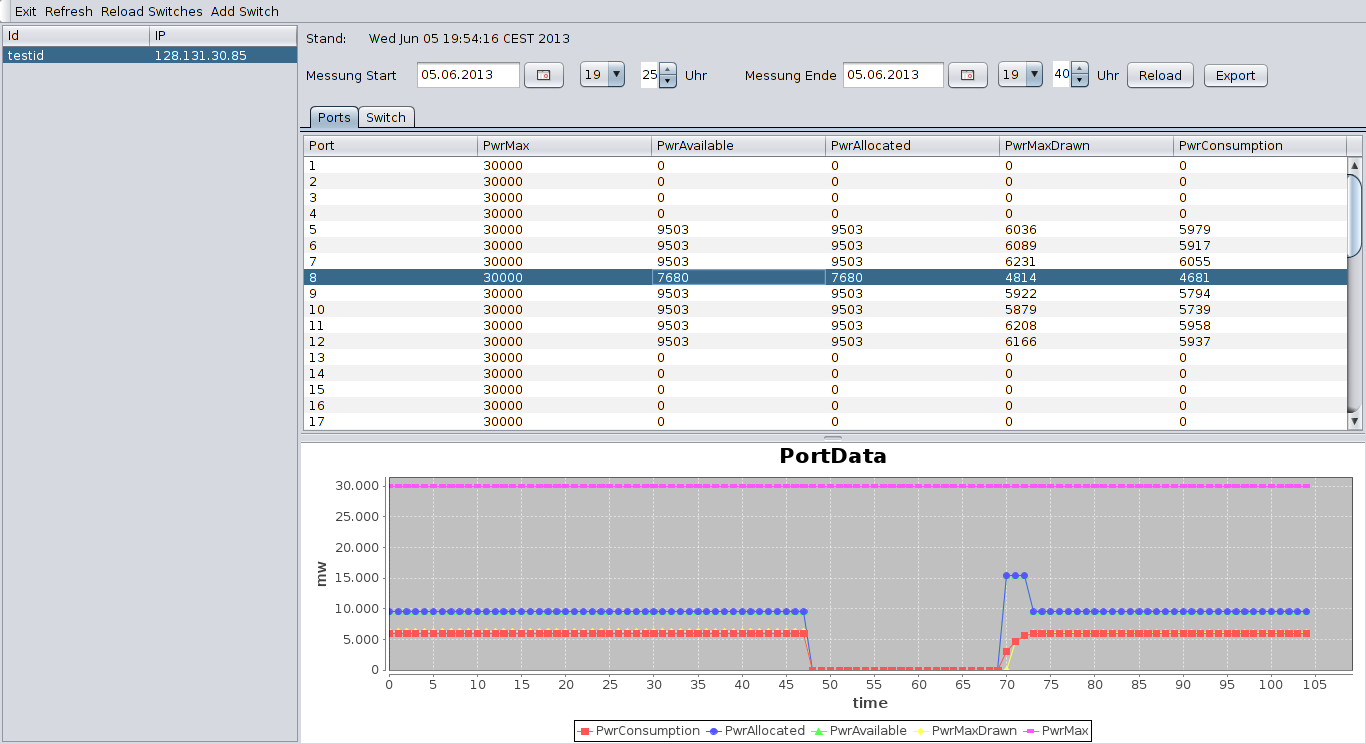
\includegraphics[width=1.0\linewidth]{figures/portDetails}
    \caption{Screenshot Verlauf Port Detail}
    \label{fig:portDetails}
\end{figure}

\subsubsection{Auswirkungen auf einen Switch}
In Abbildung \ref{fig:switchDetails} sieht man die Auswirkungen durch die Deaktivierung und anschließender Aktivierung der Ports durch das definierte Testszenario. Ähnlich wie bei der Auswirkung auf einen Port sieht auch die Auswirkung auf den Switch aus, nur das hier kumulierte Werte vorliegen. Tabelle \ref{tab:measurementAction} zeigt das Verhältnis der Messung-Nummer (die man in Abbildung \ref{fig:switchDetails} ablesen kann) zu den Aktionen welche im Szenario definiert wurden steht.

\begin{table}[h]
 \centering
 \begin{tabulary}{\textwidth}{|C|C|}
  \hline
  \textbf{Messung(en)} & \textbf{Aktion} \\
  \hline
  12 & Port 6 deaktiviert. \\
  \hline
  33-37 & Ports 10 und 11 deaktiviert. \\
  \hline
  58 & Port 40 deaktiviert. \\
  \hline
  83-87 & Port 40 aktiviert. \\
  \hline
  106-113 & Ports 10 und 11 aktiviert. \\
  \hline
  128-135 & Port 6 aktiviert. \\
  \hline
 \end{tabulary}
 \caption{Verhältnis Messung-Nummer und Aktion in Abbildung \ref{fig:switchDetails}}
 \label{tab:measurementAction}
\end{table}

\begin{figure}[h]
    \centering
    \leavevmode
    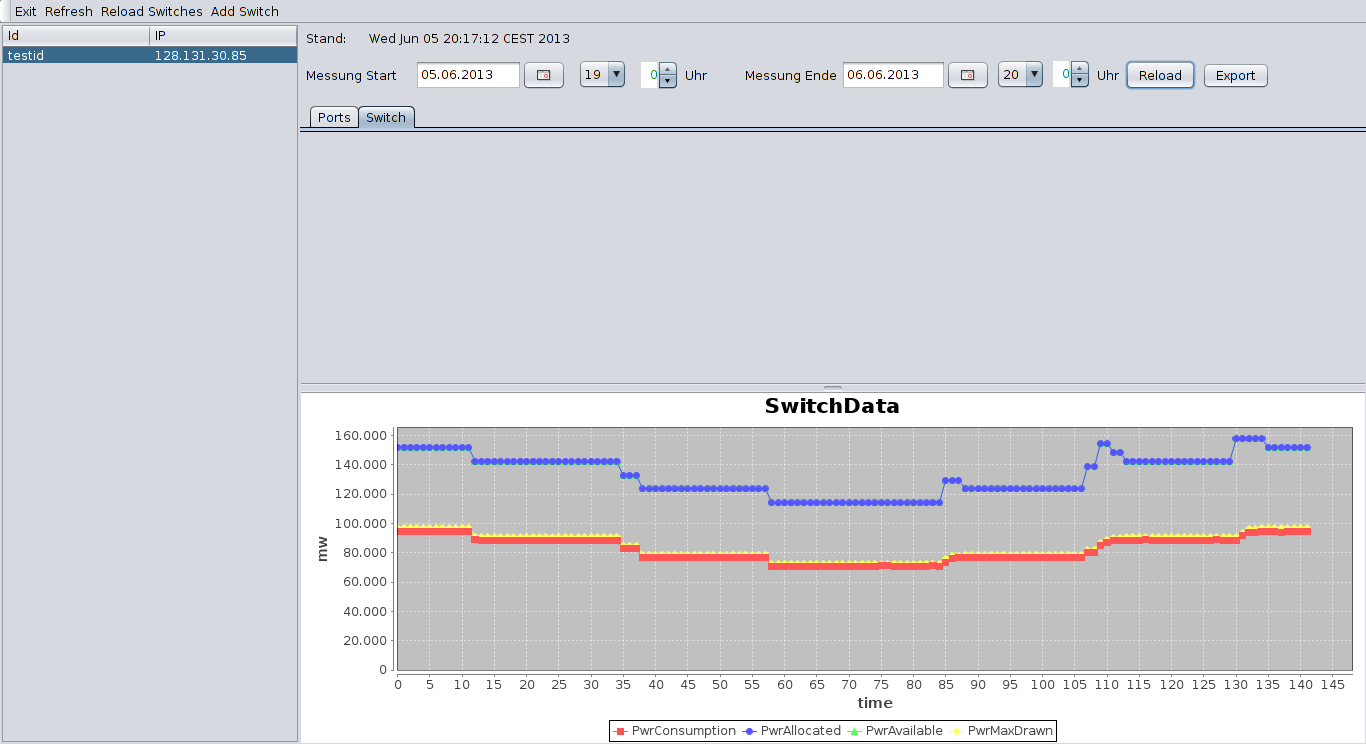
\includegraphics[width=1.0\linewidth]{figures/switchDetails}
    \caption{Screenshot Verlauf Switch Detail}
    \label{fig:switchDetails}
\end{figure}

Wie in Abbildung \ref{fig:switchDetails} gut gesehen werden kann, dauert der Prozess bis sich die Verbrauchscharakteristik wieder normalisiert hat nach dem Einschalten eines Ports deutlich länger als nach dem Ausschalten eines Ports. Die Erklärung hierfür wurde schon in den Details der Auswirkungen auf einen einzelnen Port erläutert.

\subsection{Probleme und Lösungen}
Während der Testläufe unseres Tools sind ein paar Probleme aufgetreten, welche aber alle gefunden und behoben werden konnten. Ein paar dieser Probleme und deren Lösung sind im folgenden aufgelistet:

\subsubsection*{SNMP Zugriff auf Switches}
Anfangs hatten wir das Problem, dass wir die Switches zwar per Ping erreichen konnten, jedoch kein Zugriff per SNMP möglich war. Das Problem bestand darin, dass der SNMP Service in den Switches per default deaktiviert ist. Also mussten wir zuerst den SNMP Service der Switches aktivieren.

\subsubsection*{SNMP Antworten langsamer als erwartet}
Bevor wir im Produktivsystem mit den Switches in Berührung kamen, nahmen wir an, dass SNMP Anfragen sehr schnell beantwortet wurden. Leider sind die Antworten etwas langsamer als erwartet. Dies führte zu kleineren Problemen in der Ansicht der Werte in der Tabelle beziehungsweise in den Graphen. Kleinere Anpassungen der GUI konnten Probleme hier verschwinden lassen.

Weiters ging unser Algorithmus so vor, dass sobald Messungen von einen Port zur Verfügung standen, diese sofort in die Datenbank eingespielt wurden. Dies führte dazu, dass im Switch Übersichtsgraph immer eine starke Flanke nach unten bei der neuesten Messung angezeigt wurde (da noch nicht alle Daten von jedem Switch vorhanden waren). Dies wurde behoben indem die Messungen der Ports erst dann eingespielt werden, wenn alle Daten von allen Ports geladen wurden.

\subsubsection*{Unerwartete SNMP Antworten}
Unter den Werten die wir per SNMP von einen Port auslesen, befindet sich auch ein boolscher Wert (Port aktiviert oder nicht). Jedes Port welches aktiviert war, hat einen Fehler geworfen. Nach kurzem Nachforschen wurde das Problem entdeckt: Während praktisch in der ganzen EDV der Wert 0 wahr bedeutet und 1 falsch, ist es bei diesem Wert so, dass 1 wahr und 2 falsch bedeutet. Eine kleine Anpassung in unseren SNMP Lesern lösten dieses Problem.

